%template for producing IEEE-format articles using LaTeX.
%written by Matthew Ward, CS Department, Worcester Polytechnic Institute.
%use at your own risk.  Complaints to /dev/null.
%make two column with no page numbering, default is 10 point
\documentclass[twocolumn, 10pt]{article}
\usepackage{booktabs}
\usepackage{graphicx}
\usepackage{multirow}
\usepackage{tabularx}
\usepackage{ltablex}
\usepackage{float}
% \pagestyle{empty}
    

%set dimensions of columns, gap between columns, and space between paragraphs
\setlength{\textheight}{8.75in}
\setlength{\columnsep}{2.0pc}
\setlength{\textwidth}{6.8in}
% \setlength{\footheight}{0.0in}
\setlength{\topmargin}{0.25in}
\setlength{\headheight}{0.0in}
\setlength{\headsep}{0.0in}
\setlength{\oddsidemargin}{-.19in}
\setlength{\parindent}{1pc}

%I copied stuff out of art10.sty and modified them to conform to IEEE format

\makeatletter
%as Latex considers descenders in its calculation of interline spacing,
%to get 12 point spacing for normalsize text, must set it to 10 points
\def\@normalsize{\@setsize\normalsize{12pt}\xpt\@xpt
\abovedisplayskip 10pt plus2pt minus5pt\belowdisplayskip \abovedisplayskip
\abovedisplayshortskip \z@ plus3pt\belowdisplayshortskip 6pt plus3pt
minus3pt\let\@listi\@listI} 

%need an 11 pt font size for subsection and abstract headings
\def\subsize{\@setsize\subsize{12pt}\xipt\@xipt}

%make section titles bold and 12 point, 2 blank lines before, 1 after
\def\section{\@startsection {section}{1}{\z@}{24pt plus 2pt minus 2pt}
{12pt plus 2pt minus 2pt}{\large\bf}}

%make subsection titles bold and 11 point, 1 blank line before, 1 after
\def\subsection{\@startsection {subsection}{2}{\z@}{12pt plus 2pt minus 2pt}
{12pt plus 2pt minus 2pt}{\subsize\bf}}
\makeatother



\begin{document}

%don't want date printed
\date{\today}

%make title bold and 14 pt font (Latex default is non-bold, 16 pt)
\title{\Large\bf Compiler Optimisation Coursework}

%for single author (just remove % characters)
%\author{I. M. Author \\
%  My Department \\
%  My Institute \\
%  My City, ST, zip}

%for two authors (this is what is printed)
\author{s1208506\\The University of Edinburgh}

\maketitle

%I don't know why I have to reset thispagesyle, but otherwise get page numbers
% \thispagestyle{empty}

\subsection*{\centering Abstract}
%IEEE allows italicized abstract
{\em
This report details the use of an iterative algorithm in attempting to find an optimal selection of compiler flags for GCC targetting twelve specific benchmark programs. A set of weights for each flag were continually updated to improve the execution speed over time. Results for each benchmark are presented as well as comparing each flag set over the cumulative time. For each benchmark, many flag sets were found which improved the result over -O3 and two sets were able to beat -O3 for all twelve benchmarks.
%end italics mode
}

\section{Introduction}
When compiling a program using the GCC compiler, several preset levels of optimisation are available: \texttt{-O0, -O1, -O2, -O3}. These implement a selection of \emph{compiler flags} which have been found to be almost always beneficial in improving the execution time of the resulting program. The highest level, \texttt{-O3}, is more experimental and can sometimes decrease performance over \texttt{-O2}. This is due to the difficulty in creating a single set of compiler flags which are effective for any target program.

This report describes a method for iteratively selecting additional compiler flags beyond \texttt{-O3}, in an attempt to both find an optimal set of flags for each target program as well as the best set across all of the test programs. A set of varied benchmark programs were provided as the target programs for this investigation.


\section{Evaluation Methodology}
% Selection of flags
% Weight bag algorithm
\subsection{Initial Flag Selection}
In order to reduce the problem space, a subset of all possible GCC compiler optimisation flags was selected from the official documentation page \cite{gccFlags}. The compiler options from \texttt{-O1} and \texttt{-O2} have been extensively tested so were always included in the tests. The flags in the \texttt{-O3} set are considered more experimental, so for each experiment set they were set active by default but the corresponding \texttt{-fno} flags were included in the option pool. A collection of other flags which were not in any of the \texttt{-O1}, \texttt{-O2} or \texttt{-O3} sets were also included in this option pool. Optimisation parameters (\texttt{param}) were not considered in this investigation, so all flags used their default values. In total, a pool of 65 flags was chosen.

\subsection{Flag Weighting Method}
In an effort to iteratively improve the result in subsequent runs, a flag weighting system was devised. For each benchmark program, the execution time for \texttt{-O3} was measured and used as the target time. All individual flag options were then run alone\footnote{In addition to \texttt{-O3}} for each benchmark and the resulting execution time compared against \texttt{-O3}. The results for these tests were used as the initial \emph{weight} values assigned to each flag where the weight value was equal to the integer number of milliseconds faster than \texttt{-O3}\footnote{Weights can be negative if the flag was slower than base \texttt{-O3}}.  A distinct set of weights was maintained for each benchmark in addition to an \emph{overall} set which compared the cumulative time across all 12 benchmark programs.

The hypothesis was that flags which performed well should be included more often in test sets. Therefore the next test set should be drawn from the total pool of flags based upon probabilities proportional to the current weight assigned to each flag. After a test run, the weights for all flags which were selected should be updated depending on if the execution time was greater or less than that of \texttt{-O3}. To make this system more stable, a \emph{damping factor} of 0.25 was introduced. Each flag was then increased or decreased by the execution time difference (compared to \texttt{-O3}) multiplied by 0.25. 

% A damping factor of 25\% was added

For each iteration, either the \emph{overall} set of weights or a specific benchmark is targetted and used as the probability distribution for drawing flags from the pool. The number of flags drawn was chosen to be a random integer between 2 and 50. Once a set was chosen, regardless of the target benchmark, it was run through all 12 benchmarks as per the experiment specification. Thus each iteration would update all 12 individual flag weight sets as well as the overall set.

\subsection{Experiments}
The experimental procedure followed the schedule:
\begin{enumerate}
    \item Run each benchmark for \texttt{-O0}, \texttt{-O1}, \texttt{-O2} and \texttt{-O3}. (x4)
    \item Run each flag alone as \texttt{-O3 [flag]}. (x65)
    \item Run 50 iterations of the selection algorithm targetting the \textit{overall} pool. (x50)
    \item Run 20 iterations targetting each benchmark in turn. (x240)
    \item Run 50 iterations of the selection algorithm targetting the \textit{overall} pool. (x50)
\end{enumerate}
Therefore 409 iterations were scheduled to run. However, as some flags were incompatible with each other, any selection which failed to compile or resulted in an execution output which was inconsistent with the result from \texttt{-O0} was discarded. This left 344 successful runs.



\section{Experimental Setup}
\subsection{Platform}
% Platform, how time was measured, no. runs
The experiments were all conducted on an Apple Macbook Air laptop. In an effort to reduce any processor \emph{noise}, all other programs were closed and the laptop was disconnected from the internet. Table \ref{tab:hwspecs} details the exact specification of the hardware used.

\begin{table}[ht]
    \centering
    \begin{tabular}{ll}
        \toprule
        Processor name     & Intel Core i7 (4650U)\\
        Clock Speed        & 1.7 Ghz\\
        Number of cores    & 2\\
        L2 Cache per core  & 256 KB\\
        L3 Cache           & 4 MB\\
        Main Memory        & 8 GB DDR3 @ 1600MHz \\
        \bottomrule
    \end{tabular}
    \caption{Hardware specification used in the following tests}
    \label{tab:hwspecs}
\end{table}

The operating system used was macOS High Sierra, version 10.13.2. All scripting was done using Python 3.6.4 and the version of GCC used was 7.3.0.

\subsection{Timing}
% unix time command
% real time vs user+sys
% median and confidenc intervals vs mean or just 10
It was important to accurately measure the execution time of each compiled benchmark program. Each program was run multiple times in order to average the run times and reduce the effects of noise. The mean and standard deviation were calculated but the primary method for ranking the run times was the median. For measuring the execution time of the target benchmarks, the results were expected to not be normally distributed as there is a bound on the lower run time (fastest possible execution) but the upper limit is unbounded \cite{median}. At least ten iterations were performed to comply with the provided specification. However, additional iterations were run in order to ensure that the 95\% confidence interval in the median was less than 3\% of the median wide.

The 95\% lower confidence limit was found as the $i^{th}$ value of the sorted list of execution times where $i$ was found as:
\begin{displaymath}
    i = \frac{n}{2} - \frac{ 1.96 \sqrt{n}}{2}
\end{displaymath}
Similarly, the 95\% upper confidence limit was found as the $j^{th}$ value of the sorted list where $j$ was found as:
\begin{displaymath}
    j = 1 + \frac{n}{2} + \frac{ 1.96 \sqrt{n}}{2}
\end{displaymath}

When updating the weights after each benchmark, if the median execution time for the test set fell within the lower and upper confidence bounds for \texttt{-O3}, then the result was considered equivalent to \texttt{-O3} and the weights remained unchanged.

To measure the raw timing values for each run the UNIX \texttt{time} command was used. This returns values for \emph{real}, \emph{user} and \emph{sys} time for the program under test. For the purposes of this experiment, it was decided that \emph{real} time should be used as it represents raw ``wall-clock'' time. An alternative option was to use \emph{user} + \emph{sys} time which would return the amount of time spent by the CPU actually running the process (\emph{user}) and spent in the kernel within the process (\emph{sys}). Results from some initial experiments showed that $real \approx user + sys$. If a program was able to use more than one core then it would be possible for \emph{user + sys} time to exceed \emph{real} time. As it was unknown whether any paralellisation was present in the benchmark programs or could be added via certain compiler flags, \emph{real} time was chosen, although this could potentially suffer greater effects from external CPU activity.



\section{Results}
For each benchmark, the results will be presented in a table. The median values were the key measurement for analysis. Statistics for the four base optimisation levels will be given, as well as data for the fastest flag set. The average time from all iterative flag sets is also given. A full list of flags in each fastest flag set are also listed in the appendix. 

\subsection{401.bzip2}
% chart
% \begin{figure}[]
%     \centering
%     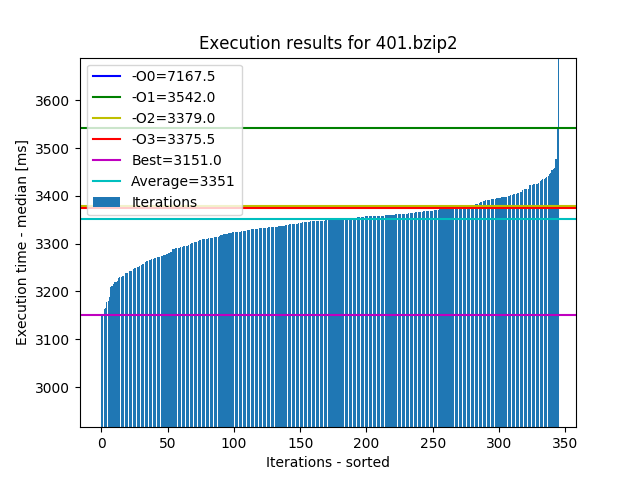
\includegraphics[width=0.5\textwidth]{../graphs/bzip2}
%     \caption{Execution results for the 401.bip2 benchmark}
%     \label{fig:bzip2_chart}
% \end{figure}

\begin{table}[H]
    \centering
    \begin{tabular}{llllll}
        \toprule
        Flag set & Mean & SD & Med. & $CI_{l}$ & $CI_{u}$ \\
        \midrule
        \texttt{-O0} &7166&68&7168&7094&7289 \\
        \texttt{-O1} &3541&23&3542&3503&3568 \\
        \texttt{-O2} &3384&26&3379&3360&3433 \\
        \texttt{-O3} &3373&37&3375&3334&3433 \\
        Fastest &3157&31&3151&3146&3183 \\
        Average &-&-&3351&-&- \\
        \bottomrule
        \multicolumn{6}{l}{\footnotesize\textbf{SD}: Standard Deviation; \textbf{Med.}: Median}\\
        \multicolumn{6}{l}{\footnotesize\textbf{$CI_{l}$}: 95\% Confidence Interval in the median lower limit;}\\
        \multicolumn{6}{l}{\footnotesize\textbf{$CI_{u}$}: 95\% Confidence Interval in the median upper limit;}\\
    \end{tabular}
    \caption{Execution time results for 401.bzip2 in ms}

    \label{tab:bzip2}
\end{table}

Results are summarised in Table \ref{tab:bzip2}.
% fastest set
The fastest set completed in 3151 ms which was 6.6\% faster than \texttt{-O3}, which completed in 3375 ms.
These flags are given in the appendix as flag set 1.
% {\scriptsize\texttt{-O3 -fsplit-loops -fbranch-probabilities -fsched-stalled-insns -fweb -fselective-scheduling -fno-predictive-commoning -floop-unroll-and-jam -fstdarg-opt -fkeep-inline-functions -funroll-loops -fno-zero-initialized-in-bss -fprefetch-loop-arrays -fno-defer-pop -floop-nest-optimize -fno-function-cse -fmerge-all-constants -flimit-function-alignment -fgcse-las -fvpt -fno-inline-functions -fsched-critical-path-heuristic -fpeel-loops -fconserve-stack -fsched-spec-load-dangerous -fipa-pta -fsched-spec-insn-heuristic -funroll-all-loops -fvariable-expansion-in-unroller -fselective-scheduling2 -fsched-group-heuristic -fsched-rank-heuristic -fmodulo-sched -fsection-anchors -fisolate-erroneous-paths-attribute -fivopts -funswitch-loops -fno-ipa-cp-clone -ftree-vectorize -freschedule-modulo-scheduled-loops -ftree-loop-im -fsched-spec-load}}.
% average time

The average execution time was 3351 ms, 0.7\% faster than \texttt{-O3}.
% best and worst flags
% \begin{figure}[]
%     \centering
%     \begin{tabular}{c}
%         \toprule
%         \textbf{Best flags} \\
%         \midrule
%         \texttt{-fbranch-probabilities} \\
%         \texttt{-fsched-stalled-insns}  \\
%         \texttt{-fisolate-erroneous-paths-attribute} \\
%         \midrule
%         \textbf{Worst flags} \\
%         \midrule
%         \texttt{-fno-inline} \\
%         \texttt{-fsched-group-heuristic} \\
%         \texttt{-fselective-scheduling2} \\
%         \bottomrule
%     \end{tabular}
%     \caption{Best and worst flags for 401.bzip2 - by final weight value}
%     \label{tab:bzip2}
% \end{figure}
% comment


\subsection{429.mcf}
% chart
% \begin{figure}[]
%     \centering
%     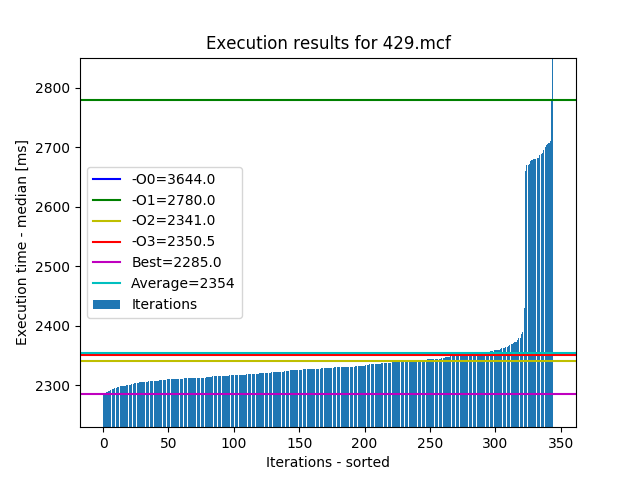
\includegraphics[width=0.5\textwidth]{../graphs/mcf}
%     \caption{Execution results for the 429.mcf benchmark}
%     \label{fig:mcf_chart}
% \end{figure}

\begin{table}[H]
    \centering
    \begin{tabular}{llllll}
        \toprule
        Flag set & Mean & SD & Med. & $CI_{l}$ & $CI_{u}$ \\
        \midrule
        \texttt{-O0} &3643&59&3644&3612&3694 \\
        \texttt{-O1} &2873&253&2780&2752&2829 \\
        \texttt{-O2} &2339&33&2341&2311&2376 \\
        \texttt{-O3} &2350&27&2351&2324&2391 \\
        Fastest &2282&27&2285&2248&2313 \\
        Average &-&-&2354&-&- \\
        \bottomrule
    \end{tabular}
    \caption{Execution time results for 429.mcf in ms}
    \label{tab:mcf}
\end{table}
Results are summarised in Table \ref{tab:mcf}.
% fastest set
The fastest set completed in 2285 ms which was 2.8\% faster than \texttt{-O3}, which completed in 2351 ms. \texttt{-O2} was also faster than \texttt{-O3} with a time of 2341 ms, but the fastest set was still 2.4\% faster.
This fastest flag set is given in the appendix as flag set 2.
% The flags were just {\scriptsize\texttt{-O3 -fsection-anchors}}.
% average time

The average execution time was 2354 ms, 0.13\% slower than \texttt{-O3}.
% best and worst flags
% \begin{figure}[]
%     \centering
%     \begin{tabular}{c}
%         \toprule
%         \textbf{Best flags} \\
%         \midrule
%         \texttt{-fbranch-probabilities} \\
%         \texttt{-fsched-stalled-insns}  \\
%         \texttt{-fisolate-erroneous-paths-attribute} \\
%         \midrule
%         \textbf{Worst flags} \\
%         \midrule
%         \texttt{-fno-inline} \\
%         \texttt{-fsched-group-heuristic} \\
%         \texttt{-fselective-scheduling2} \\
%         \bottomrule
%     \end{tabular}
%     \caption{Best and worst flags for 429.mcf - by final weight value}
%     \label{tab:bzip2}
% \end{figure}
% comment



\subsection{433.milc}
% chart
% \begin{figure}[]
%     \centering
%     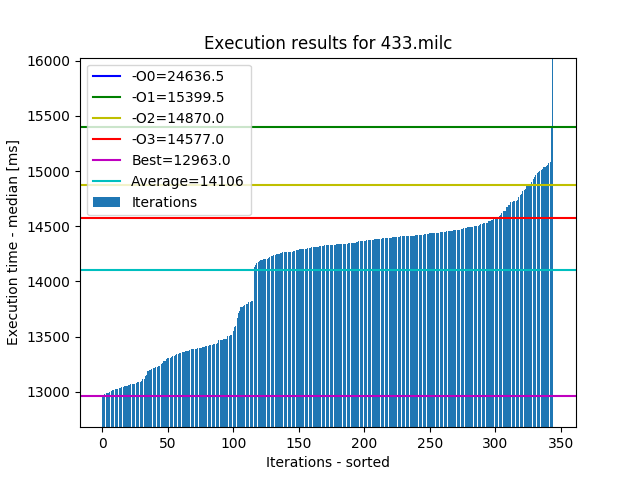
\includegraphics[width=0.5\textwidth]{../graphs/milc}
%     \caption{Execution results for the 433.milc benchmark}
%     \label{fig:milc_chart}
% \end{figure}

\begin{table}[H]
    \centering
    \begin{tabular}{llllll}
        \toprule
        Flag set & Mean & SD & Med. & $CI_{l}$ & $CI_{u}$ \\
        \midrule
        \texttt{-O0} &24670&136&24636&24524&24858 \\
        \texttt{-O1} &15321&233&15400&15159&15486 \\
        \texttt{-O2} &14807&331&14870&14582&15017 \\
        \texttt{-O3} &14544&337&14577&14325&14748 \\
        Fastest &13039&218&12963&12916&13237  \\
        Average &-&-&14106&-&- \\
        \bottomrule
    \end{tabular}
    \caption{Execution time results for 433.milc in ms}
    \label{tab:milc}
\end{table}
Results are summarised in Table \ref{tab:milc}.
% fastest set
The fastest set completed in 12963 ms which was 11.1\% faster than \texttt{-O3}, which completed in 14577 ms.
This flag set is given in the appendix as set 3.
% The flags were just {\scriptsize\texttt{-O3 -fselective-scheduling -funroll-loops -fprofile-use -fsched-last-insn-heuristic -fstdarg-opt -fsched-rank-heuristic -flimit-function-alignment -fselective-scheduling2 -fmodulo-sched -floop-nest-optimize -fsched-spec-load-dangerous -fipa-pta -fgcse-after-reload -fprofile-correction -fkeep-static-functions -fprefetch-loop-arrays -flto -fbtr-bb-exclusive -funswitch-loops -fkeep-inline-functions -floop-unroll-and-jam}}.
% average time
The average execution time was 14106 ms, 3.2\% faster than \texttt{-O3}.
% comment



\subsection{445.gobmk}
% chart
% \begin{figure}[]
%     \centering
%     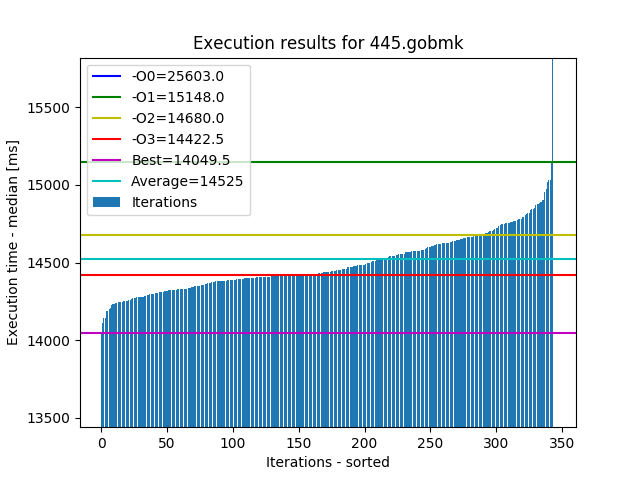
\includegraphics[width=0.5\textwidth]{../graphs/gobmk}
%     \caption{Execution results for the 445.gobmk benchmark}
%     \label{fig:gobmk_chart}
% \end{figure}

\begin{table}[H]
    \centering
    \begin{tabular}{llllll}
        \toprule
        Flag set & Mean & SD & Med. & $CI_{l}$ & $CI_{u}$ \\
        \midrule
        \texttt{-O0} &25867&729&25603&25576&25988 \\
        \texttt{-O1} &15145&65&15148&15071&15252 \\
        \texttt{-O2} &14658&70&14680&14559&14739 \\
        \texttt{-O3} &14422&53&14423&14350&14499 \\
        Fastest &14058&52&14050&14004&14176  \\
        Average &-&-&14525&-&- \\
        \bottomrule
    \end{tabular}
    \caption{Execution time results for 445.gobmk in ms}
    \label{tab:gobmk}
\end{table}
Results are summarised in Table \ref{tab:gobmk}.
% fastest set
The fastest set completed in 14050 ms which was 2.6\% faster than \texttt{-O3}, which completed in 14423 ms.
This flag set is listed in the appendix as set 4.
% The flags were {\scriptsize\texttt{-O3 -ftree-vectorize -fisolate-erroneous-paths-attribute -flto -flimit-function-alignment -fcx-limited-range}}.

% average time
The average execution time was 14525 ms, 0.71\% slower than \texttt{-O3}.
% comment




\subsection{456.hmmer}
% chart
% \begin{figure}[]
%     \centering
%     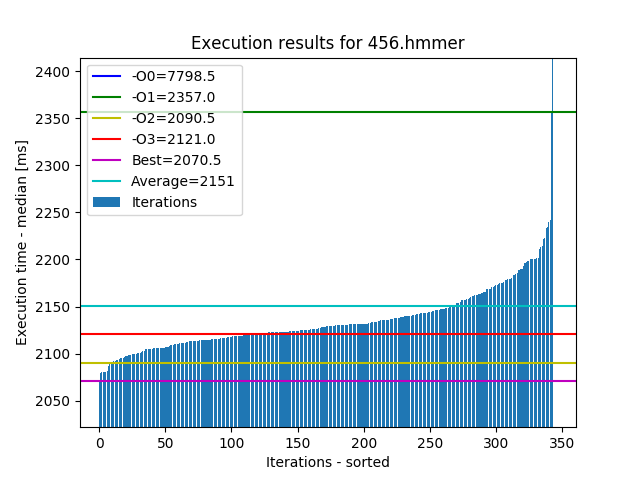
\includegraphics[width=0.5\textwidth]{../graphs/hmmer}
%     \caption{Execution results for the 456.hmmer benchmark}
%     \label{fig:hmmer_chart}
% \end{figure}

\begin{table}[H]
    \centering
    \begin{tabular}{llllll}
        \toprule
        Flag set & Mean & SD & Med. & $CI_{l}$ & $CI_{u}$ \\
        \midrule
        \texttt{-O0} &7801&45&7799&7754&7879 \\
        \texttt{-O1} &2377&46&2357&2352&2420 \\
        \texttt{-O2} &2099&41&2091&2070&2123 \\
        \texttt{-O3} &2140&55&2121&2110&2164 \\
        Fastest &2086&50&2071&2057&2118  \\
        Average &-&-&2151&-&- \\
        \bottomrule
    \end{tabular}
    \caption{Execution time results for 456.hmmer in ms}
    \label{tab:hmmer}
\end{table}
Results are summarised in Table \ref{tab:hmmer}.
% fastest set
The fastest set completed in 2017 ms which was 4.9\% faster than \texttt{-O3}, which completed in 2121 ms. \texttt{-O2} was also faster than \texttt{-O3}, with a time of 2091 ms, but the fastest set was still 0.96\% faster.
% mention o2?
This flag set is listed in the appendix as set 5.
% The flags were {\scriptsize\texttt{-O3 -fisolate-erroneous-paths-attribute -fno-ira-share-spill-slots -fsched-stalled-insns-dep -fno-zero-initialized-in-bss -flto -fcx-limited-range -fprofile-use -fselective-scheduling2 -fstdarg-opt -fipa-pta -fgcse-sm -fsched-dep-count-heuristic -fsplit-loops -fsched-group-heuristic -frename-registers -freschedule-modulo-scheduled-loops}}.

% average time
The average execution time was 2151 ms, 1.4\% slower than \texttt{-O3}.
% comment



\subsection{458.sjeng}
% chart
% \begin{figure}[]
%     \centering
%     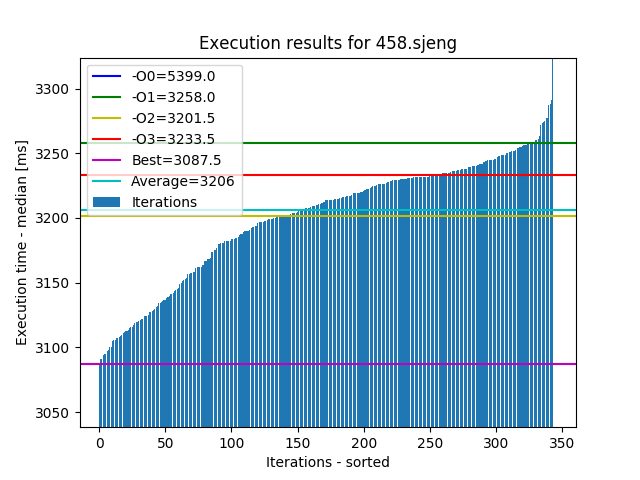
\includegraphics[width=0.5\textwidth]{../graphs/sjeng}
%     \caption{Execution results for the 458.sjeng benchmark}
%     \label{fig:sjeng_chart}
% \end{figure}

\begin{table}[H]
    \centering
    \begin{tabular}{llllll}
        \toprule
        Flag set & Mean & SD & Med. & $CI_{l}$ & $CI_{u}$ \\
        \midrule
        \texttt{-O0} &5415&50&5399&5385&5458 \\
        \texttt{-O1} &3258&28&3258&3226&3298 \\
        \texttt{-O2} &3201&24&3202&3190&3243 \\
        \texttt{-O3} &3236&20&3234&3218&3269 \\
        Fastest &3099&28&3088&3072&3143  \\
        Average &-&-&3206&-&- \\
        \bottomrule
    \end{tabular}
    \caption{Execution time results for 458.sjeng in ms}
    \label{tab:sjeng}
\end{table}
Results are summarised in Table \ref{tab:sjeng}.
% fastest set
The fastest set completed in 3088 ms which was 4.8\% faster than \texttt{-O3}, which completed in 3243 ms.  \texttt{-O2} was also faster than \texttt{-O3} with a time of 3202 ms, but the fastest set was still 3.6\% faster.
% mention o2?
This set of flags is given in the appendix as flag set 6.
% The flags were {\scriptsize\texttt{-O3 -fselective-scheduling -fno-ira-share-save-slots -flto -flive-range-shrinkage -fsched-stalled-insns -fsched-last-insn-heuristic -fweb -fdevirtualize-speculatively -fvpt -fgcse-sm -fno-function-cse -floop-parallelize-all -fprofile-use -fgcse-after-reload -fivopts -fstdarg-opt -flimit-function-alignment -fno-ipa-cp-clone -fprefetch-loop-arrays -funroll-all-loops -fconserve-stack -fkeep-inline-functions -fsched2-use-superblocks -freschedule-modulo-scheduled-loops -fsched-spec-insn-heuristic -fkeep-static-functions -fvariable-expansion-in-unroller -fsched-pressure -fno-zero-initialized-in-bss -fsched-spec-load}}.

% average time
The average execution time was 3206 ms, 1.1\% faster than \texttt{-O3}.
% comment



\subsection{462.libquantum}
% chart
% \begin{figure}[]
%     \centering
%     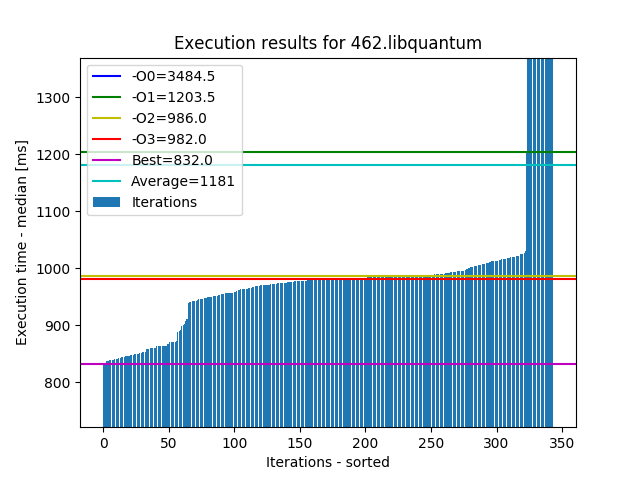
\includegraphics[width=0.5\textwidth]{../graphs/libquantum}
%     \caption{Execution results for the 462.libquantum benchmark}
%     \label{fig:libquantum_chart}
% \end{figure}

\begin{table}[H]
    \centering
    \begin{tabular}{llllll}
        \toprule
        Flag set & Mean & SD & Med. & $CI_{l}$ & $CI_{u}$ \\
        \midrule
        \texttt{-O0} &3475&28&3485&3451&3509 \\
        \texttt{-O1} &1207&20&1204&1191&1227 \\
        \texttt{-O2} &986&14&986&972&1000 \\
        \texttt{-O3} &984&15&982&973&998 \\
        Fastest &835&12&832&827&847  \\
        Average &-&-&1181&-&- \\
        \bottomrule
    \end{tabular}
    \caption{Execution time results for 462.libquantum in ms}
    \label{tab:quant}
\end{table}
Results are summarised in Table \ref{tab:quant}.
% fastest set
The fastest set completed in 832 ms which was 15.3\% faster than \texttt{-O3}, which completed in 982 ms.
% mention o2?
This set of flags is given in the appendix as set 7.
% The flags were {\scriptsize\texttt{-O3 -fgcse-after-reload -floop-unroll-and-jam -fkeep-inline-functions -fbtr-bb-exclusive -fbranch-target-load-optimize -fivopts -fsched-spec-load-dangerous -funroll-all-loops -fpeel-loops -fsched2-use-superblocks -fprefetch-loop-arrays -flto -fweb -fselective-scheduling -fmerge-all-constants -fipa-pta -fno-ira-share-spill-slots -flimit-function-alignment -fno-function-cse -fgcse-sm -fsched-critical-path-heuristic -floop-nest-optimize -frename-registers -fbranch-probabilities -fsched-pressure -fcx-limited-range -fsched-spec-load -fsched-spec-insn-heuristic -ftree-loop-ivcanon -funroll-loops -fno-zero-initialized-in-bss -ftree-vectorize -fgcse-las}}.

% average time
The average execution time was 1181 ms, 20\% slower than \texttt{-O3}. Indeed, several flag sets were in fact slower than \texttt{-O0}.
% comment



\subsection{464.h264ref}
% chart
% \begin{figure}[]
%     \centering
%     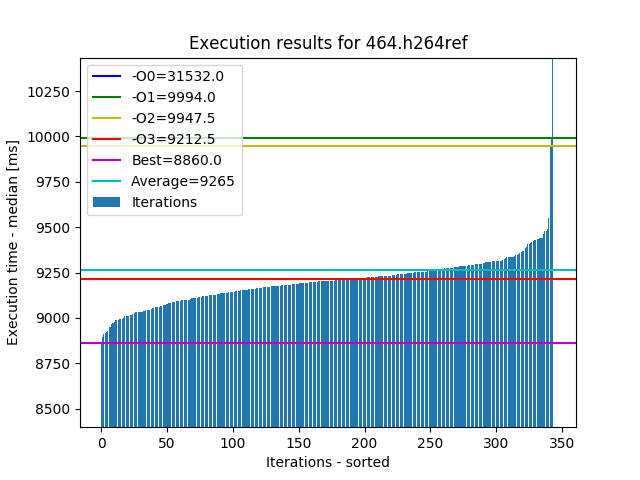
\includegraphics[width=0.5\textwidth]{../graphs/h264ref}
%     \caption{Execution results for the 464.h264ref benchmark}
%     \label{fig:h264ref_chart}
% \end{figure}

\begin{table}[H]
    \centering
    \begin{tabular}{llllll}
        \toprule
        Flag set & Mean & SD & Med. & $CI_{l}$ & $CI_{u}$ \\
        \midrule
        \texttt{-O0} &31771&587&31532&31440&31668 \\
        \texttt{-O1} &10050&183&9994&9962&10055 \\
        \texttt{-O2} &9968&83&9948&9876&10130 \\
        \texttt{-O3} &9210&57&9213&9136&9314 \\
        Fastest &8840&54&8860&8770&8903  \\
        Average &-&-&9265&-&- \\
        \bottomrule
    \end{tabular}
    \caption{Execution time results for 464.h264ref in ms}
    \label{tab:ref}
\end{table}
Results are summarised in Table \ref{tab:ref}.
% fastest set
The fastest set completed in 8860 ms which was 3.8\% faster than \texttt{-O3}, which completed in 9213 ms.
% mention o2?
This flag set is given in the appendix as set 8.
% The flags were {\scriptsize\texttt{-O3 -fno-predictive-commoning -fno-function-cse -fsched-rank-heuristic -fmodulo-sched -flto -funswitch-loops -ftree-loop-ivcanon -fsched-dep-count-heuristic -fisolate-erroneous-paths-attribute -fsched-spec-load -fsched-stalled-insns -fcx-limited-range -fno-zero-initialized-in-bss -funroll-all-loops -flive-range-shrinkage -fpeel-loops -fgcse-sm -fweb -fgcse-after-reload -fsched-critical-path-heuristic -fivopts -fvariable-expansion-in-unroller -fno-defer-pop -fipa-pta -fsched-stalled-insns-dep -fno-ira-share-save-slots -fsched-pressure -fbranch-probabilities}}.

% average time
The average execution time was 9265 ms, 0.56\% slower than \texttt{-O3}.
% comment




\subsection{470.lbm}
% chart
% \begin{figure}[]
%     \centering
%     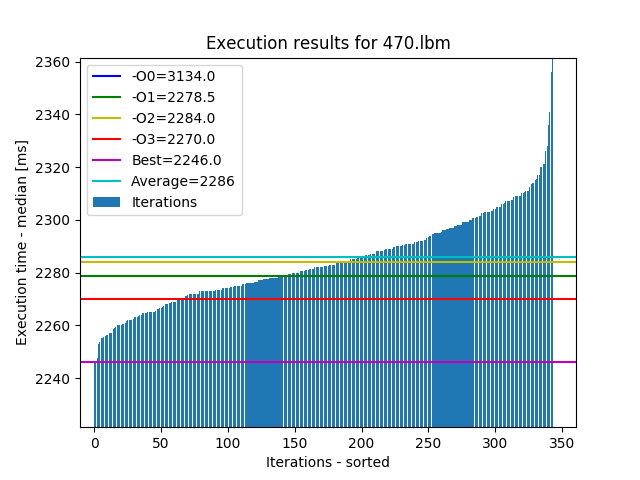
\includegraphics[width=0.5\textwidth]{../graphs/lbm}
%     \caption{Execution results for the 470.lbm benchmark}
%     \label{fig:lbm_chart}
% \end{figure}

\begin{table}[H]
    \centering
    \begin{tabular}{llllll}
        \toprule
        Flag set & Mean & SD & Med. & $CI_{l}$ & $CI_{u}$ \\
        \midrule
        \texttt{-O0} &3137&37&3134&3106&3172 \\
        \texttt{-O1} &2277&23&2279&2248&2314 \\
        \texttt{-O2} &2279&25&2284&2255&2312 \\
        \texttt{-O3} &2270&21&2270&2240&2305 \\
        Fastest &2256&22&2246&2242&2288  \\
        Average &-&-&2286&-&- \\
        \bottomrule
    \end{tabular}
    \caption{Execution time results for 470.lbm in ms}
    \label{tab:lbm}
\end{table}
Results are summarised in Table \ref{tab:lbm}.
% fastest set
The fastest set completed in 2246 ms which was 1.1\% faster than \texttt{-O3}, which completed in 2270 ms.
% mention o2?
This flag set is given in the appendix as set 9.
% The flags were {\scriptsize\texttt{-O3 -fmerge-all-constants -floop-unroll-and-jam -fsched-spec-load-dangerous -fvariable-expansion-in-unroller -floop-parallelize-all -fgcse-las -fisolate-erroneous-paths-attribute -fselective-scheduling -fsplit-loops -flimit-function-alignment -fmodulo-sched -fno-ira-share-save-slots -fsched2-use-superblocks -fweb -fno-zero-initialized-in-bss -fpeel-loops -flive-range-shrinkage -fbranch-target-load-optimize2 -fivopts -fgcse-after-reload -fbtr-bb-exclusive -fconserve-stack -fstdarg-opt -fsched-stalled-insns -fno-function-cse -fsection-anchors -freschedule-modulo-scheduled-loops -frename-registers -fdevirtualize-speculatively -fkeep-static-functions -fno-defer-pop -fno-predictive-commoning -fsched-stalled-insns-dep -fsched-last-insn-heuristic -fno-ipa-cp-clone -ftree-vectorize -ftree-loop-ivcanon -fsched-spec-insn-heuristic -fipa-pta -fprefetch-loop-arrays -fprofile-correction -fsched-dep-count-heuristic -fno-ira-share-spill-slots -fsched-rank-heuristic -floop-nest-optimize}}.

% average time
The average execution time was 2286 ms, 0.70\% slower than \texttt{-O3}.
% comment



\subsection{h263dec}
% comment - didn't compile
This benchmark could not compile due to issues in the code. It was omitted from the investigation.

\subsection{h263enc}
% chart
% \begin{figure}[]
%     \centering
%     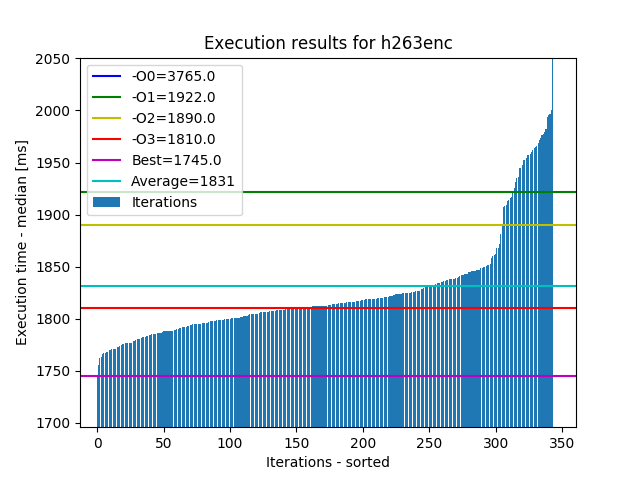
\includegraphics[width=0.5\textwidth]{../graphs/h263enc}
%     \caption{Execution results for the h263enc benchmark}
%     \label{fig:h263enc_chart}
% \end{figure}

\begin{table}[H]
    \centering
    \begin{tabular}{llllll}
        \toprule
        Flag set & Mean & SD & Med. & $CI_{l}$ & $CI_{u}$ \\
        \midrule
        \texttt{-O0} &3770&42&3765&3739&3836 \\
        \texttt{-O1} &1932&29&1922&1912&1966 \\
        \texttt{-O2} &1902&21&1890&1884&1929 \\
        \texttt{-O3} &1811&18&1810&1797&1829 \\
        Fastest &1752&21&1745&1736&1786  \\
        Average &-&-&1831&-&- \\
        \bottomrule
    \end{tabular}
    \caption{Execution time results for h263enc in ms}
    \label{tab:hdec}
\end{table}
Results are summarised in Table \ref{tab:hdec}.
% fastest set
The fastest set completed in 1745 ms which was 3.6\% faster than \texttt{-O3}, which completed in 1810 ms.
% mention o2?
These flags are given in flag set 10 in the appendix.
% The flags were {\scriptsize\texttt{-O3 -flto -fsched-stalled-insns -fcx-limited-range -fgcse-sm -fprefetch-loop-arrays -floop-parallelize-all -fno-ira-share-spill-slots}}.

% average time
The average execution time was 1831 ms, 1.2\% slower than \texttt{-O3}.
% comment


\subsection{mpeg2dec}
% chart
% \begin{figure}[]
%     \centering
%     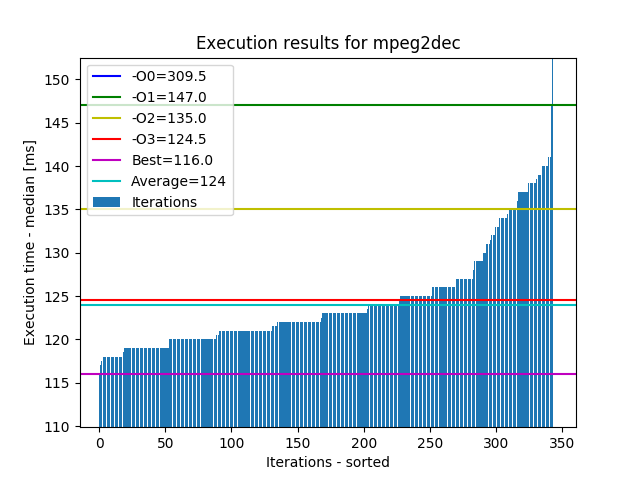
\includegraphics[width=0.5\textwidth]{../graphs/mpeg2dec}
%     \caption{Execution results for the mpeg2dec benchmark}
%     \label{fig:mpeg2dec_chart}
% \end{figure}

\begin{table}[H]
    \centering
    \begin{tabular}{llllll}
        \toprule
        Flag set & Mean & SD & Med. & $CI_{l}$ & $CI_{u}$ \\
        \midrule
        \texttt{-O0} &313&14&310&307&315 \\
        \texttt{-O1} &150&10&147&146&150 \\
        \texttt{-O2} &138&12&135&133&137 \\
        \texttt{-O3} &126&8&125&123&126 \\
        Fastest &120&12&116&115&118  \\
        Average &-&-&124&-&- \\
        \bottomrule
    \end{tabular}
    \caption{Execution time results for mpeg2dec in ms}
    \label{tab:mdec}
\end{table}
Results are summarised in Table \ref{tab:mdec}.
% fastest set
The fastest set completed in 116 ms which was 7.2\% faster than \texttt{-O3}, which completed in 125 ms.
% mention o2?
These flags are given in flag set 11 in the appendix.
% The flags were {\scriptsize\texttt{-O3 -fsched2-use-superblocks -floop-nest-optimize -fsched-pressure -fno-defer-pop -floop-interchange -fno-predictive-commoning -fivopts -fgcse-sm -fsched-stalled-insns-dep -fpeel-loops -fsched-spec-load-dangerous -fsplit-loops -fkeep-static-functions -floop-parallelize-all -fselective-scheduling -fno-ira-share-save-slots -fno-function-cse -funroll-all-loops -fsched-spec-insn-heuristic -flimit-function-alignment -fcx-limited-range -fvpt -fgcse-after-reload -fdevirtualize-speculatively}}.

% average time
The average execution time was 124 ms, 0.8\% faster than \texttt{-O3}.
% comment




\subsection{mpeg2enc}
% chart
% \begin{figure}[]
%     \centering
%     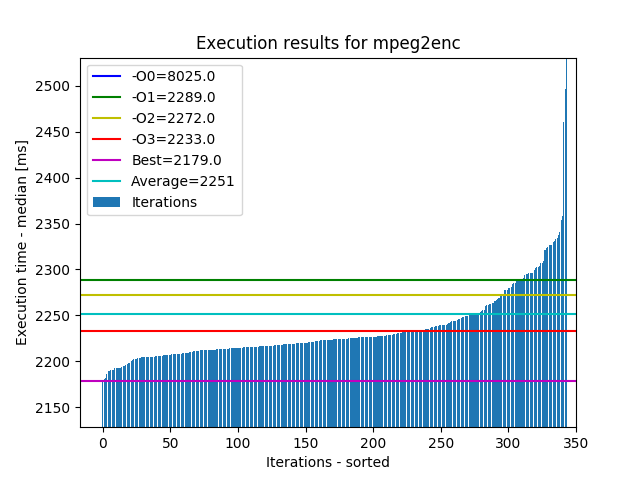
\includegraphics[width=0.5\textwidth]{../graphs/mpeg2enc}
%     \caption{Execution results for the mpeg2enc benchmark}
%     \label{fig:mpeg2enc_chart}
% \end{figure}

\begin{table}[H]
    \centering
    \begin{tabular}{llllll}
        \toprule
        Flag set & Mean & SD & Med. & $CI_{l}$ & $CI_{u}$ \\
        \midrule
        \texttt{-O0} &8097&206&8025&7965&8128 \\
        \texttt{-O1} &2291&21&2289&2266&2328 \\
        \texttt{-O2} &2278&29&2272&2255&2316 \\
        \texttt{-O3} &2231&31&2233&2206&2271 \\
        Fastest &2194&26&2179&2172&2224  \\
        Average &-&-&2251&-&- \\
        \bottomrule
    \end{tabular}
    \caption{Execution time results for mpeg2enc in ms}
    \label{tab:menc}
\end{table}
Results are summarised in Table \ref{tab:menc}.
% fastest set
The fastest set completed in 2179 ms which was 2.4\% faster than \texttt{-O3}, which completed in 2233 ms.
% mention o2?
These flags are given in the appendix as flag set 12.
% The flags were {\scriptsize\texttt{-O3 -fno-function-cse -fvpt -fsched-group-heuristic -flive-range-shrinkage -fivopts -fsched-stalled-insns -fgcse-las -ftree-parallelize-loops=16 -fgcse-after-reload -funroll-loops -fno-inline -fno-zero-initialized-in-bss -fsched2-use-superblocks -fsched-pressure -fsched-spec-insn-heuristic -fipa-pta -fbranch-target-load-optimize2 -fkeep-inline-functions -fprefetch-loop-arrays -fisolate-erroneous-paths-attribute -ftree-vectorize -fmodulo-sched -funswitch-loops -fdevirtualize-speculatively -ftree-loop-ivcanon -fgcse-sm -fweb -fsched-rank-heuristic -fno-inline-functions}}.

% average time
The average execution time was 2251 ms, 0.8\% slower than \texttt{-O3}.
% comment


\subsection{Overall}
% chart
% \begin{figure}[]
%     \centering
%     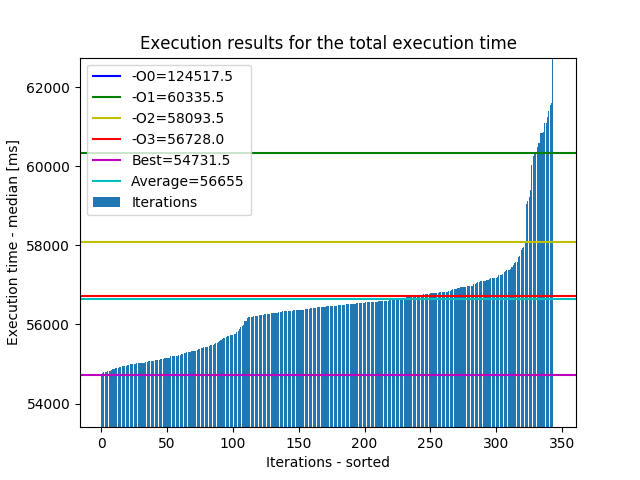
\includegraphics[width=0.5\textwidth]{../graphs/overall}
%     \caption{Execution results for all benchmarks cumulatively}
%     \label{fig:overall_chart}
% \end{figure}

\begin{table}[H]
    \centering
    \begin{tabular}{lll}
        \toprule
        Flag set & Mean & Med. \\
        \midrule
        \texttt{-O0} &125146&124518 \\
        \texttt{-O1} &60436&60336 \\
        \texttt{-O2} &58056&58094 \\
        \texttt{-O3} &56713&56728 \\
        Fastest &54757&54731  \\
        Average &-&56655\\
        \bottomrule
    \end{tabular}
    \caption{Execution time results for the cumulative execution time of all 12 benchmarks in ms}
    \label{tab:ov}
\end{table}
Results are summarised in Table \ref{tab:ov}.
% fastest set
The fastest set completed in 54731 ms which was 3.5\% faster than \texttt{-O3}, which completed in 56728 ms.
% mention o2?
% average time
These flags are given in the appendix as flag set 13.
% The flags were {\scriptsize\texttt{-O3 -flto -fselective-scheduling -fgcse-sm -floop-unroll-and-jam -flimit-function-alignment -fmodulo-sched -fbranch-target-load-optimize2 -flive-range-shrinkage -fbranch-probabilities -ftree-loop-ivcanon -fno-predictive-commoning -fno-function-cse -fprefetch-loop-arrays -fsched-group-heuristic -floop-parallelize-all -fsched-pressure -fno-zero-initialized-in-bss -fgcse-after-reload -fsched-stalled-insns-dep -fconserve-stack -ftree-parallelize-loops=16 -fsched-critical-path-heuristic -fcx-limited-range -fkeep-inline-functions -fvariable-expansion-in-unroller -frename-registers -fsection-anchors -fbtr-bb-exclusive -fprofile-use -fsplit-loops -fno-ira-share-save-slots -ftree-loop-im -funroll-all-loops -fsched-last-insn-heuristic -fsched-spec-load-dangerous -fkeep-static-functions -fmerge-all-constants -fdevirtualize-speculatively -fweb -fstdarg-opt -fno-ira-share-spill-slots -fbranch-target-load-optimize -floop-interchange}}.

This is the ``fastest set of flags across all programs'' but was only faster than \texttt{-O3} in 10 of the 12 benchmarks.

The average execution time was 56655 ms, 0.13\% faster than \texttt{-O3}.

There were two flag sets which beat \texttt{-O3} in all 12 benchmarks. These were {\texttt{-O3 -fcx-limited-range}}, which had a cumulative time of 56230 ms and another set, given as flag set 14 of the appendix,
% {\scriptsize\texttt{-O3 -fselective-scheduling -fsection-anchors -fprefetch-loop-arrays -fdevirtualize-speculatively -fsched-dep-count-heuristic -fweb -fisolate-erroneous-paths-attribute -fpeel-loops -fbranch-target-load-optimize2 -fno-defer-pop -fsched-stalled-insns-dep -fmerge-all-constants -fbtr-bb-exclusive -ftree-loop-ivcanon -fsched-stalled-insns -fno-ira-share-spill-slots -floop-unroll-and-jam -fcx-limited-range -flto -fsched2-use-superblocks -fno-function-cse -frename-registers -fvariable-expansion-in-unroller -fivopts -fgcse-after-reload -floop-interchange -fmodulo-sched -fno-predictive-commoning -fsched-spec-insn-heuristic -fsched-spec-load-dangerous}} 
which had a cumulative time of 54865 ms.

A summary of the relative performance of the fastest and average flag sets against \texttt{-O3} is given in Table \ref{tab:sum}.

\begin{table}[H]
    \centering
    \begin{tabular}{lllll}
        \toprule
        Benchmark & \texttt{-O2} & \texttt{-O3} & Fastest & Average \\
        \midrule
        libquantum & 986 & 982 & -15.3\% & +20\%\\ 
        milc & 14870 & 14577 & -11.1\% & -3.2\%\\
        mpeg2dec & 135 & 125 & -7.2\% & -0.80\%\\
        bzip2 & 3379 & 3375 & -6.6\% & +0.70\%\\
        hmmer & 2091 & 2121 & -4.9\% & +1.4\%\\
        sjeng & 3202 & 3234 & -4.8\% & -1.1\%\\
        h264ref & 9948 & 9213 & -3.8\% & +0.56\%\\
        h263enc & 1890 & 1810 & -3.6\% & +1.2\%\\
        mcf & 2341 & 2311 & -2.8\% & +0.13\%\\
        gobmk & 14680 & 14423 & -2.6\% & +0.71\%\\
        mpeg2enc & 2272 & 2233 & -2.4\% & +0.80\%\\
        lbm & 2284 & 2270 & -1.1\% & +0.70\%\\
        \midrule
        \emph{overall} & 58094 & 56728 & -3.5\% & -0.13\%\\
        \bottomrule
    \end{tabular}
    \caption{Summary of the fastest and average flag sets vs. \texttt{-O3}}
    \label{tab:sum}
\end{table}
% comment

\section{Analysis and Discussion}
\subsection{Observations from the results}
% Overview discussion
In all benchmarks, the iterative weight-based algorithm was successful in finding multiple flag sets which produced a faster execution time of the benchmark over \texttt{-O3}. It was interesting to note that of the 344 flag sets tested, only two were consistently faster than \texttt{-O3} for all 12 benchmarks. This highlights the difficulty in finding one \textit{best} set of compiler flags for all possible programs. 

% Anomaly in libquantum
For most benchmarks, the average result of all flag sets was close to the performance of \texttt{-O3}. This was to be expected, as they all start from the baseline settings of \texttt{-O3}. An interesting anomaly was in the \textit{libquantum} benchmark where the average was 20\% worse. There were some flag sets which produced disasterous results, even slower than \texttt{-O0}. However, each flag that was included in some of the worst sets, with execution times around 4900 ms, was also present in some of the best sets with execution times around 850 ms. The raw timing data was examined to ensure that these results were not consecutive as this may have indicated a period of external CPU noise. These 4000+ ms runs were evenly spread throughout which suggests this was not the issue. Instead, it implies that it was the combinations of certain flags which produced these issues. 

% Best and worst speed-ups found
The level of success for the best performing flag sets was also drastically different for each benchmark. Improvements of over 10\% were achieved for the \emph{libquantum} and \emph{milc} benchmarks while a speedup of only 1.1\% was found for the \emph{lbm} benchmark. It is notable that \emph{libquantum} had both the best improvement with its fastest set and the worst performance on average. Compare this to \emph{lbm} which featured a minor change in both cases. This suggests, at least for the chosen flag pool in this experiment, that some programs are more invariant to compilation techniques while others have greater scope for performance alterations.

% Also noticable with the difference between o0 o1
Similar variability can be seen in the speed-up from \texttt{-O0} to \texttt{-03} as shown in Table \ref{tab:compben}. However, there is no strong correlation between the benchmarks which benefit the most from the \texttt{-03} optimisations and those which benefit the most from the custom optimisations. 

\begin{table}[H]
    \centering
    \begin{tabular}{lll}
        \toprule
        Benchmark & \texttt{-O3} vs. \texttt{-O0} & Fastest vs. \texttt{-O3} \\
        \midrule
        libquantum & -72\%  & -15.3\% \\ 
        milc & -41\%  & -11.1\%   \\
        mpeg2dec & -60\% & -7.2\%    \\
        bzip2 & -35\%  & -6.6\%     \\
        hmmer & -73\% & -4.9\%     \\
        sjeng & -40\%  & -4.8\%     \\
        h264ref & -71\%  & -3.8\%   \\
        h263enc & -52\%  & -3.6\%   \\
        mcf & -35\% &  -2.8\%       \\
        gobmk & -44\%  & -2.6\%   \\
        mpeg2enc & -72\%  & -2.4\%  \\
        lbm & -28\%  & -1.1\%       \\
        \midrule
        \emph{overall} & -54\% & -3.5\%\\
        \bottomrule
    \end{tabular}
    \caption{Compilation benefits comparison}
    \label{tab:compben}
\end{table}

\subsection{The Weight-based Algorithm}
% The weight system allows for specific good and bad flags to be found
The use of the weight system allowed for the relative performance of each flag for each benchmark to be assessed. Although this was not perfect, as a great flag could be pushed down the rankings due to frequently being drawn along with poor flags. Consistently high performing flags were \texttt{-flto} and \texttt{-fprofile-use} while consistently poor flags were \texttt{-fno-inline-functions} and \texttt{-fno-inline}. Even with these however, there were certain benchmarks where they had the opposite effect. 

% Best and worst weight
Across all flag weight sets, the highest value achieved was \texttt{-flto} on the \emph{milc} benchmark with a weight of 29934. The lowest value achieved was \texttt{-ftree-parallelize-loops=16} on the \emph{libquantum} benchmark with a weight of -21199.

% improvements to algorithm
To further improve the results, some additional work could be done to the search algorithm. A major flaw in the weight-based system is that a potentially good flag could, by chance, be included in a set with one or more highly deterimental flags early in the process. If this set then resulted in a very negative result, then the potentially strong flag will have its weight reduced to an unrepresentative value and it would then be unlikely to be drawn again.
% could run more iterations
More iterations targetting each benchmark would also be beneficial in further improving the results.

% could add weighting system to no flags as maybe correlation in number of flags to performance?
Another extension would be in extending the weight system to the flag set size parameter. Instead of just randomly selecting a set size each iteration, the sizes could also be weighted to investigate if smaller or larger set sizes were more likely to result in an effective set. From the results, this was also a benchmark specific property. For example, the majority of the best performing benchmarks for \emph{mcf} were a single flag whereas for \emph{libquantum}, most had over 40.

\section{Summary and Conclusions}
This investigation has proven that using iterative compilation techniques is effective at reducing the execution time for various benchmark programs. A significant perfromance increase over the standard \texttt{-O3} flag setting is possible when targetting a single program. However, difficulties in finding one set of compiler flags which are effective for any arbitrary program were highlighted. 

The specific flags included, and the number of flags in the fastest set, were significantly variable for each of the benchmarks investigated. This leads to the conclusion that the method of iterative compilation for a specific target program is essential in achieving an optimal result.

While analysing the results, it became clear that there were many complexities involved with selecting compiler optimisation flags, even for a single target program. Flags could produce good results alone but when used in combination, produce highly negative results and vice versa. It was also observed that some programs were more invariant to improvements from the compiler than others.

If optimum performance is sought for a target program then an iterative compilation system would be a valuable exercise.



\begin{thebibliography}{9}
    
    % \bibitem{key:foo}
    % I. M. Author, 
    % ``Some Related Article I Wrote,''
    % {\em Some Fine Journal}, Vol. 17, pp. 1-100, 1987.
    
    % \bibitem{foo:baz}
    % A. N. Expert, 
    % {\em A Book He Wrote,}
    % His Publisher, 1989.
    
    \bibitem{gccFlags}
    Free Software Foundation, Inc.
    ``3.10 Options That Control Optimization,''
    \emph{Using the GNU Compiler Collection (GCC)}
    https://gcc.gnu.org/onlinedocs/gcc/Optimize-Options.html
    
    \bibitem{median}
    Torsten Hoefler,
    ``How many measurements do you need to report a performance number?''
    https://htor.inf.ethz.ch/blog/index.php/2016/04/14/how-many-measurements-do-you-need-to-report-a-performance-number/
    
\end{thebibliography}

\onecolumn
\section*{Appendix: Full flag sets}
The full flag sets mentioned in the report are listed here.

% \begin{table}[h]
    \centering
    \begin{tabularx}{\textwidth}{llX}
        \toprule
        Flag set & Benchmark & Flags \\
        \midrule
        \endhead
        1 & bzip2 & \texttt{-O3 -fsplit-loops -fbranch-probabilities -fsched-stalled-insns -fweb -fselective-scheduling -fno-predictive-commoning -floop-unroll-and-jam -fstdarg-opt -fkeep-inline-functions -funroll-loops -fno-zero-initialized-in-bss -fprefetch-loop-arrays -fno-defer-pop -floop-nest-optimize -fno-function-cse -fmerge-all-constants -flimit-function-alignment -fgcse-las -fvpt -fno-inline-functions -fsched-critical-path-heuristic -fpeel-loops -fconserve-stack -fsched-spec-load-dangerous -fipa-pta -fsched-spec-insn-heuristic -funroll-all-loops -fvariable-expansion-in-unroller -fselective-scheduling2 -fsched-group-heuristic -fsched-rank-heuristic -fmodulo-sched -fsection-anchors -fisolate-erroneous-paths-attribute -fivopts -funswitch-loops -fno-ipa-cp-clone -ftree-vectorize -freschedule-modulo-scheduled-loops -ftree-loop-im -fsched-spec-load} \\
        \midrule
        2 & mcf & \texttt{-O3 -fsection-anchors}\\
        \midrule
        3 & milc & \texttt{-O3 -fselective-scheduling -funroll-loops -fprofile-use -fsched-last-insn-heuristic -fstdarg-opt -fsched-rank-heuristic -flimit-function-alignment -fselective-scheduling2 -fmodulo-sched -floop-nest-optimize -fsched-spec-load-dangerous -fipa-pta -fgcse-after-reload -fprofile-correction -fkeep-static-functions -fprefetch-loop-arrays -flto -fbtr-bb-exclusive -funswitch-loops -fkeep-inline-functions -floop-unroll-and-jam} \\
        \midrule
        4 & gobmk & \texttt{-O3 -ftree-vectorize -fisolate-erroneous-paths-attribute -flto -flimit-function-alignment -fcx-limited-range} \\
        \midrule
        5 & hmmer & \texttt{-O3 -fisolate-erroneous-paths-attribute -fno-ira-share-spill-slots -fsched-stalled-insns-dep -fno-zero-initialized-in-bss -flto -fcx-limited-range -fprofile-use -fselective-scheduling2 -fstdarg-opt -fipa-pta -fgcse-sm -fsched-dep-count-heuristic -fsplit-loops -fsched-group-heuristic -frename-registers -freschedule-modulo-scheduled-loops} \\
        \midrule
        6 & sjeng & \texttt{-O3 -fselective-scheduling -fno-ira-share-save-slots -flto -flive-range-shrinkage -fsched-stalled-insns -fsched-last-insn-heuristic -fweb -fdevirtualize-speculatively -fvpt -fgcse-sm -fno-function-cse -floop-parallelize-all -fprofile-use -fgcse-after-reload -fivopts -fstdarg-opt -flimit-function-alignment -fno-ipa-cp-clone -fprefetch-loop-arrays -funroll-all-loops -fconserve-stack -fkeep-inline-functions -fsched2-use-superblocks -freschedule-modulo-scheduled-loops -fsched-spec-insn-heuristic -fkeep-static-functions -fvariable-expansion-in-unroller -fsched-pressure -fno-zero-initialized-in-bss -fsched-spec-load} \\
        \midrule
        7 & libquantum & \texttt{-O3 -fgcse-after-reload -floop-unroll-and-jam -fkeep-inline-functions -fbtr-bb-exclusive -fbranch-target-load-optimize -fivopts -fsched-spec-load-dangerous -funroll-all-loops -fpeel-loops -fsched2-use-superblocks -fprefetch-loop-arrays -flto -fweb -fselective-scheduling -fmerge-all-constants -fipa-pta -fno-ira-share-spill-slots -flimit-function-alignment -fno-function-cse -fgcse-sm -fsched-critical-path-heuristic -floop-nest-optimize -frename-registers -fbranch-probabilities -fsched-pressure -fcx-limited-range -fsched-spec-load -fsched-spec-insn-heuristic -ftree-loop-ivcanon -funroll-loops -fno-zero-initialized-in-bss -ftree-vectorize -fgcse-las}\\
        \midrule
        8 & h264ref & \texttt{-O3 -fno-predictive-commoning -fno-function-cse -fsched-rank-heuristic -fmodulo-sched -flto -funswitch-loops -ftree-loop-ivcanon -fsched-dep-count-heuristic -fisolate-erroneous-paths-attribute -fsched-spec-load -fsched-stalled-insns -fcx-limited-range -fno-zero-initialized-in-bss -funroll-all-loops -flive-range-shrinkage -fpeel-loops -fgcse-sm -fweb -fgcse-after-reload -fsched-critical-path-heuristic -fivopts -fvariable-expansion-in-unroller -fno-defer-pop -fipa-pta -fsched-stalled-insns-dep -fno-ira-share-save-slots -fsched-pressure -fbranch-probabilities} \\
        \midrule
        9 & lbm & \texttt{-O3 -fmerge-all-constants -floop-unroll-and-jam -fsched-spec-load-dangerous -fvariable-expansion-in-unroller -floop-parallelize-all -fgcse-las -fisolate-erroneous-paths-attribute -fselective-scheduling -fsplit-loops -flimit-function-alignment -fmodulo-sched -fno-ira-share-save-slots -fsched2-use-superblocks -fweb -fno-zero-initialized-in-bss -fpeel-loops -flive-range-shrinkage -fbranch-target-load-optimize2 -fivopts -fgcse-after-reload -fbtr-bb-exclusive -fconserve-stack -fstdarg-opt -fsched-stalled-insns -fno-function-cse -fsection-anchors -freschedule-modulo-scheduled-loops -frename-registers -fdevirtualize-speculatively -fkeep-static-functions -fno-defer-pop -fno-predictive-commoning -fsched-stalled-insns-dep -fsched-last-insn-heuristic -fno-ipa-cp-clone -ftree-vectorize -ftree-loop-ivcanon -fsched-spec-insn-heuristic -fipa-pta -fprefetch-loop-arrays -fprofile-correction -fsched-dep-count-heuristic -fno-ira-share-spill-slots -fsched-rank-heuristic -floop-nest-optimize}\\
        \midrule
        10 & h263enc & \texttt{-O3 -flto -fsched-stalled-insns -fcx-limited-range -fgcse-sm -fprefetch-loop-arrays -floop-parallelize-all -fno-ira-share-spill-slots} \\
        \midrule
        11 & mpeg2dec & \texttt{-O3 -fsched2-use-superblocks -floop-nest-optimize -fsched-pressure -fno-defer-pop -floop-interchange -fno-predictive-commoning -fivopts -fgcse-sm -fsched-stalled-insns-dep -fpeel-loops -fsched-spec-load-dangerous -fsplit-loops -fkeep-static-functions -floop-parallelize-all -fselective-scheduling -fno-ira-share-save-slots -fno-function-cse -funroll-all-loops -fsched-spec-insn-heuristic -flimit-function-alignment -fcx-limited-range -fvpt -fgcse-after-reload -fdevirtualize-speculatively} \\
        \midrule
        12 & mpeg2enc & \texttt{-O3 -fno-function-cse -fvpt -fsched-group-heuristic -flive-range-shrinkage -fivopts -fsched-stalled-insns -fgcse-las -ftree-parallelize-loops=16 -fgcse-after-reload -funroll-loops -fno-inline -fno-zero-initialized-in-bss -fsched2-use-superblocks -fsched-pressure -fsched-spec-insn-heuristic -fipa-pta -fbranch-target-load-optimize2 -fkeep-inline-functions -fprefetch-loop-arrays -fisolate-erroneous-paths-attribute -ftree-vectorize -fmodulo-sched -funswitch-loops -fdevirtualize-speculatively -ftree-loop-ivcanon -fgcse-sm -fweb -fsched-rank-heuristic -fno-inline-functions} \\
        \midrule
        13 & overall & \texttt{-O3 -flto -fselective-scheduling -fgcse-sm -floop-unroll-and-jam -flimit-function-alignment -fmodulo-sched -fbranch-target-load-optimize2 -flive-range-shrinkage -fbranch-probabilities -ftree-loop-ivcanon -fno-predictive-commoning -fno-function-cse -fprefetch-loop-arrays -fsched-group-heuristic -floop-parallelize-all -fsched-pressure -fno-zero-initialized-in-bss -fgcse-after-reload -fsched-stalled-insns-dep -fconserve-stack -ftree-parallelize-loops=16 -fsched-critical-path-heuristic -fcx-limited-range -fkeep-inline-functions -fvariable-expansion-in-unroller -frename-registers -fsection-anchors -fbtr-bb-exclusive -fprofile-use -fsplit-loops -fno-ira-share-save-slots -ftree-loop-im -funroll-all-loops -fsched-last-insn-heuristic -fsched-spec-load-dangerous -fkeep-static-functions -fmerge-all-constants -fdevirtualize-speculatively -fweb -fstdarg-opt -fno-ira-share-spill-slots -fbranch-target-load-optimize -floop-interchange} \\
        \midrule
        14 & consistent & \texttt{-O3 -fselective-scheduling -fsection-anchors -fprefetch-loop-arrays -fdevirtualize-speculatively -fsched-dep-count-heuristic -fweb -fisolate-erroneous-paths-attribute -fpeel-loops -fbranch-target-load-optimize2 -fno-defer-pop -fsched-stalled-insns-dep -fmerge-all-constants -fbtr-bb-exclusive -ftree-loop-ivcanon -fsched-stalled-insns -fno-ira-share-spill-slots -floop-unroll-and-jam -fcx-limited-range -flto -fsched2-use-superblocks -fno-function-cse -frename-registers -fvariable-expansion-in-unroller -fivopts -fgcse-after-reload -floop-interchange -fmodulo-sched -fno-predictive-commoning -fsched-spec-insn-heuristic -fsched-spec-load-dangerous} \\
        \bottomrule
        \caption{Full flag sets, included in the appendix due to their length}
    \end{tabularx}
    \label{tab:flag_sets}
% \end{table}

% \twocolumn
% \section*{Appendix: Execution time plots}
% \begin{figure}[htp]
%     \centering
%     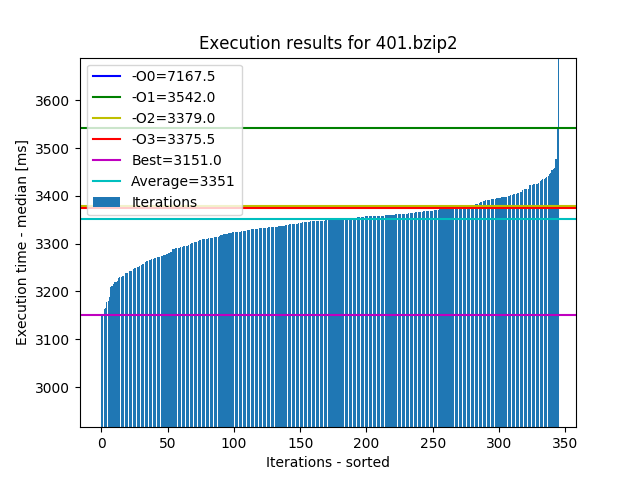
\includegraphics[width=0.49\textwidth]{../graphs/bzip2}
%     \caption{Results for the 401.bip2 benchmark}
%     \label{fig:bzip2_chart}
% \end{figure}
% \begin{figure}[htp]
%     \centering
%     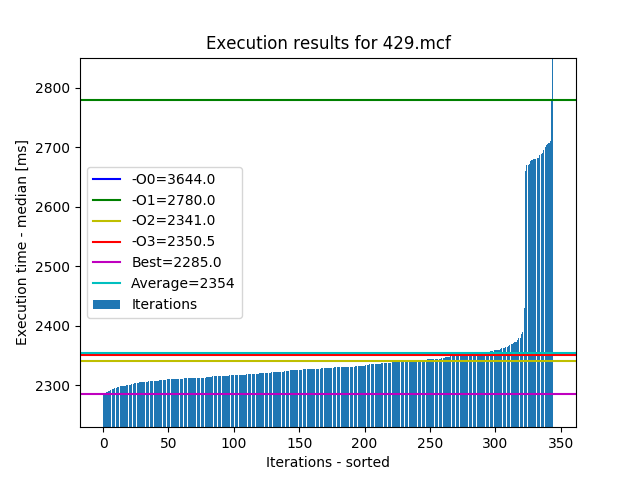
\includegraphics[width=0.49\textwidth]{../graphs/mcf}
%     \caption{Results for the 429.mcf benchmark}
%     \label{fig:mcf_chart}
% \end{figure}
% \begin{figure}[htp]
%     \centering
%     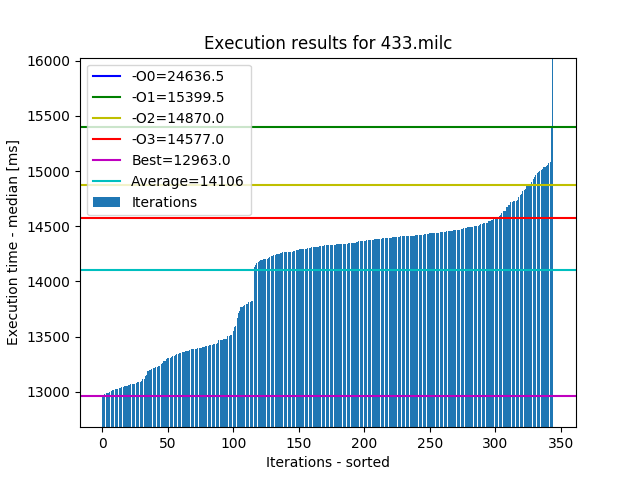
\includegraphics[width=0.49\textwidth]{../graphs/milc}
%     \caption{Results for the 433.milc benchmark}
%     \label{fig:milc_chart}
% \end{figure}
% \begin{figure}[htp]
%     \centering
%     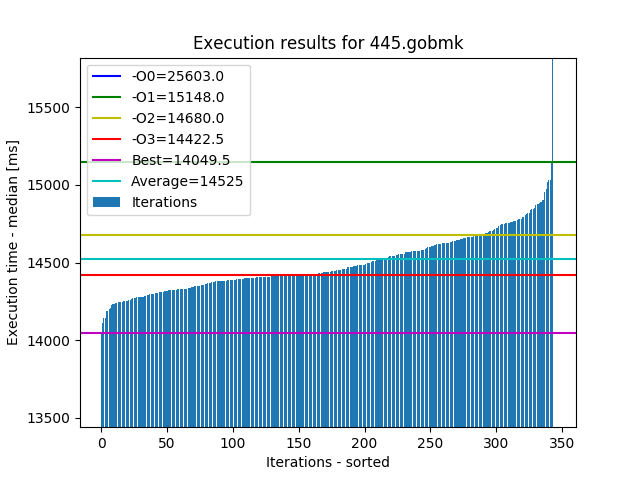
\includegraphics[width=0.49\textwidth]{../graphs/gobmk}
%     \caption{Results for the 445.gobmk benchmark}
%     \label{fig:gobmk_chart}
% \end{figure}
% \begin{figure}[htp]
%     \centering
%     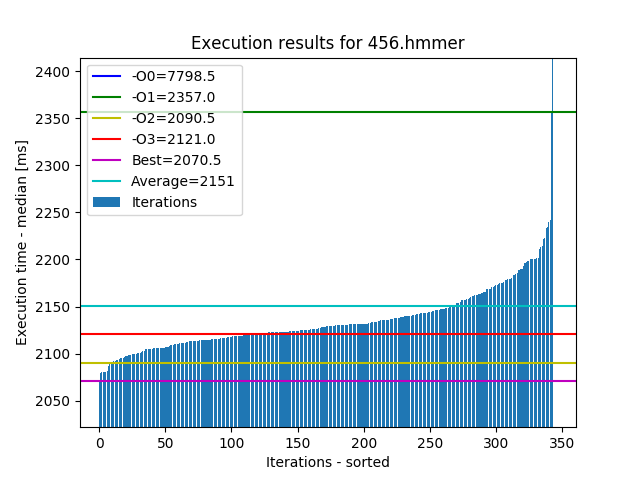
\includegraphics[width=0.49\textwidth]{../graphs/hmmer}
%     \caption{Results for the 456.hmmer benchmark}
%     \label{fig:hmmer_chart}
% \end{figure}
% \begin{figure}[htp]
%     \centering
%     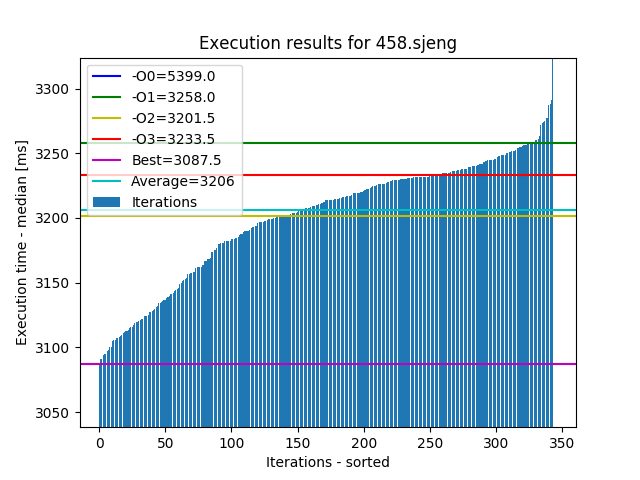
\includegraphics[width=0.49\textwidth]{../graphs/sjeng}
%     \caption{Results for the 458.sjeng benchmark}
%     \label{fig:sjeng_chart}
% \end{figure}
% \begin{figure}[htp]
%     \centering
%     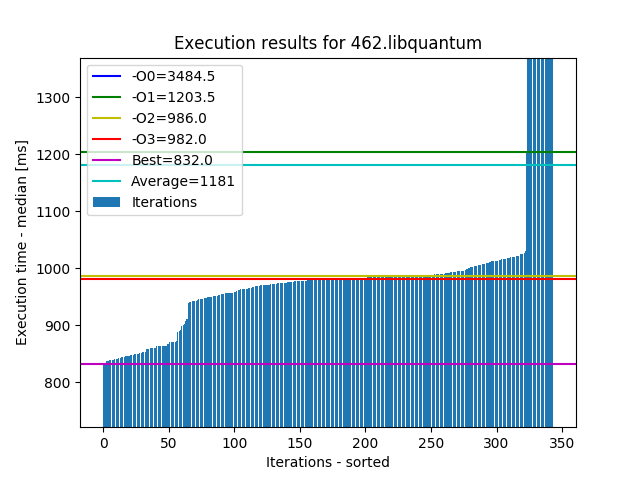
\includegraphics[width=0.49\textwidth]{../graphs/libquantum}
%     \caption{Results for the 462.libquantum benchmark}
%     \label{fig:libquantum_chart}
% \end{figure}
% \begin{figure}[htp]
%     \centering
%     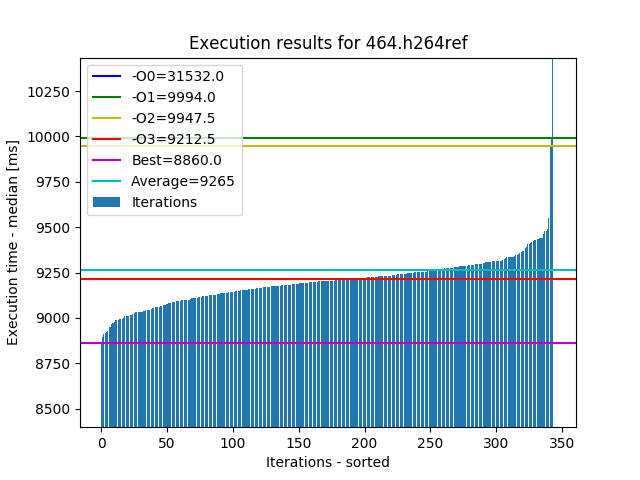
\includegraphics[width=0.49\textwidth]{../graphs/h264ref}
%     \caption{Results for the 464.h264ref benchmark}
%     \label{fig:h264ref_chart}
% \end{figure}
% \begin{figure}[htp]
%     \centering
%     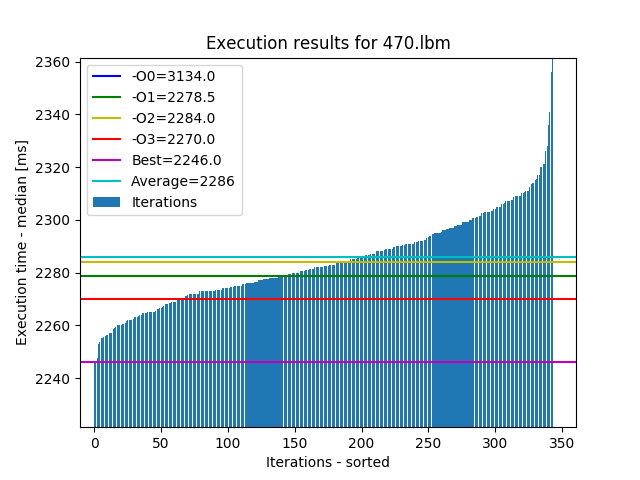
\includegraphics[width=0.49\textwidth]{../graphs/lbm}
%     \caption{Results for the 470.lbm benchmark}
%     \label{fig:lbm_chart}
% \end{figure}
% \begin{figure}[htp]
%     \centering
%     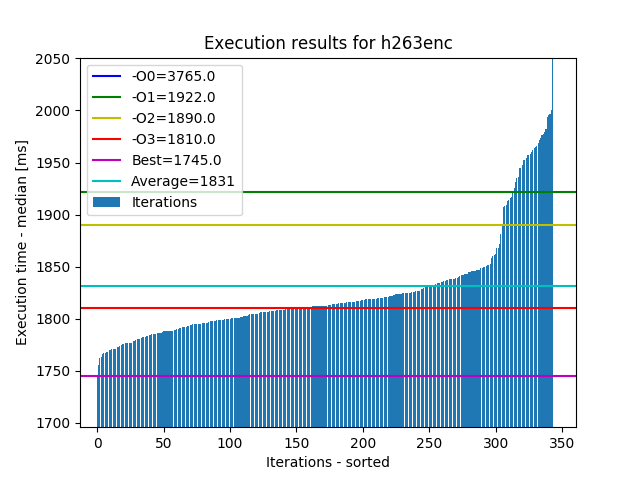
\includegraphics[width=0.49\textwidth]{../graphs/h263enc}
%     \caption{Results for the h263enc benchmark}
%     \label{fig:h263enc_chart}
% \end{figure}
% \begin{figure}[htp]
%     \centering
%     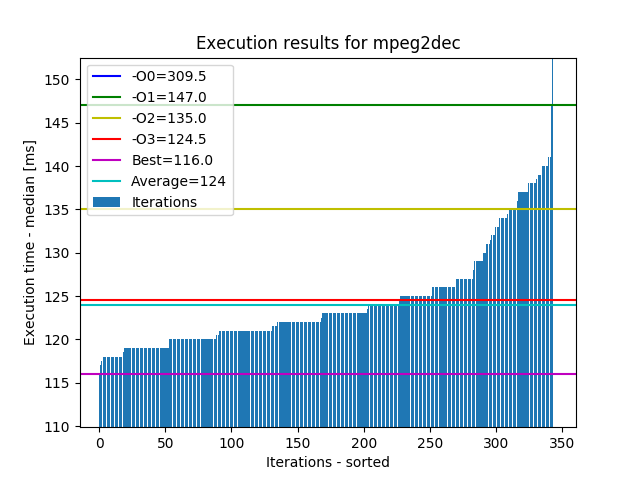
\includegraphics[width=0.49\textwidth]{../graphs/mpeg2dec}
%     \caption{Results for the mpeg2dec benchmark}
%     \label{fig:mpeg2dec_chart}
% \end{figure}
% \begin{figure}[htp]
%     \centering
%     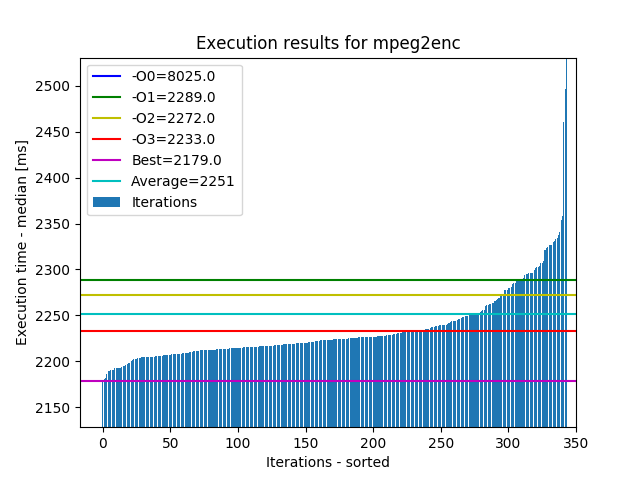
\includegraphics[width=0.49\textwidth]{../graphs/mpeg2enc}
%     \caption{Results for the mpeg2enc benchmark}
%     \label{fig:mpeg2enc_chart}
% \end{figure}
% \begin{figure}[htp]
%     \centering
%     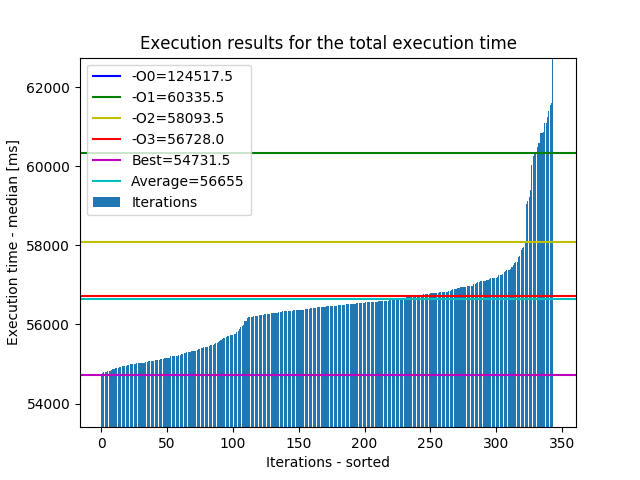
\includegraphics[width=0.49\textwidth]{../graphs/overall}
%     \caption{Results for all benchmarks cumulatively}
%     \label{fig:overall_chart}
% \end{figure}

\end{document}
